\chapter{The LHC and CMS Experiment}
\label{sec:cms}

\section{The LHC}

The Large Hadron Collider (LHC)~\cite{Evans:2008zzb}, located at CERN just outside Geneva, is a synchrotron measuring 27 km in circumference, installed in the tunnel previously used by the Large Electron-Positron (LEP) accelerator \cite{203828}. 
Upon design, its primary purpose was to provide collisions between proton beams, generating center-of-mass energies ($\sqrt{s}$) of up to 14 TeV and an instantaneous luminosity of approximately $10^{34}$ cm$^{−2}$s$^{−1}$. 
Fig~\ref{fig:CERN_Schematic} illustrates the arrangement of the LHC and the CERN accelerator complex. 
Protons are supplied to the LHC through a sequence of accelerators: Linac4 (Linac2 pre-2020), Proton Synchrotron Booster (PSB), Proton Synchrotron, and Super Proton Synchrotron (SPS), that successively raise the energies of the protons to 50 MeV, 1.4 GeV, 25 GeV, and 450 GeV respectively. 
When the final energy has been achieved, the SPS injects bunched protons into the LHC's beam pipes as two counter-rotating beams. 
Each bunch containing over $10^11$ protons, with each one separated by 25 ns and each beam consists of 2808 bunches. 
The protons are accelerated to collision energy using eight 400 MHz radio frequency (RF) cavities and kept in a circular trajectory with 1232 niobium-titanium superconducting dipole magnets. 
These magnets must be maintained at their operating temperature of 1.9 K to generate magnetic fields up to 8.4 T, requiring the use of superfluid helium. 
The bunches are collided at four intersections point surrounded by the ALICE~\cite{ALICE:2008ngc}, ATLAS~\cite{ATLAS:2008xda}, CMS~\cite{CMS_Setup} and LHCb~\cite{LHCb:2008vvz} detectors, at a collision rate of 40 MHz. \\

\begin{figure}[t]
    \centering
    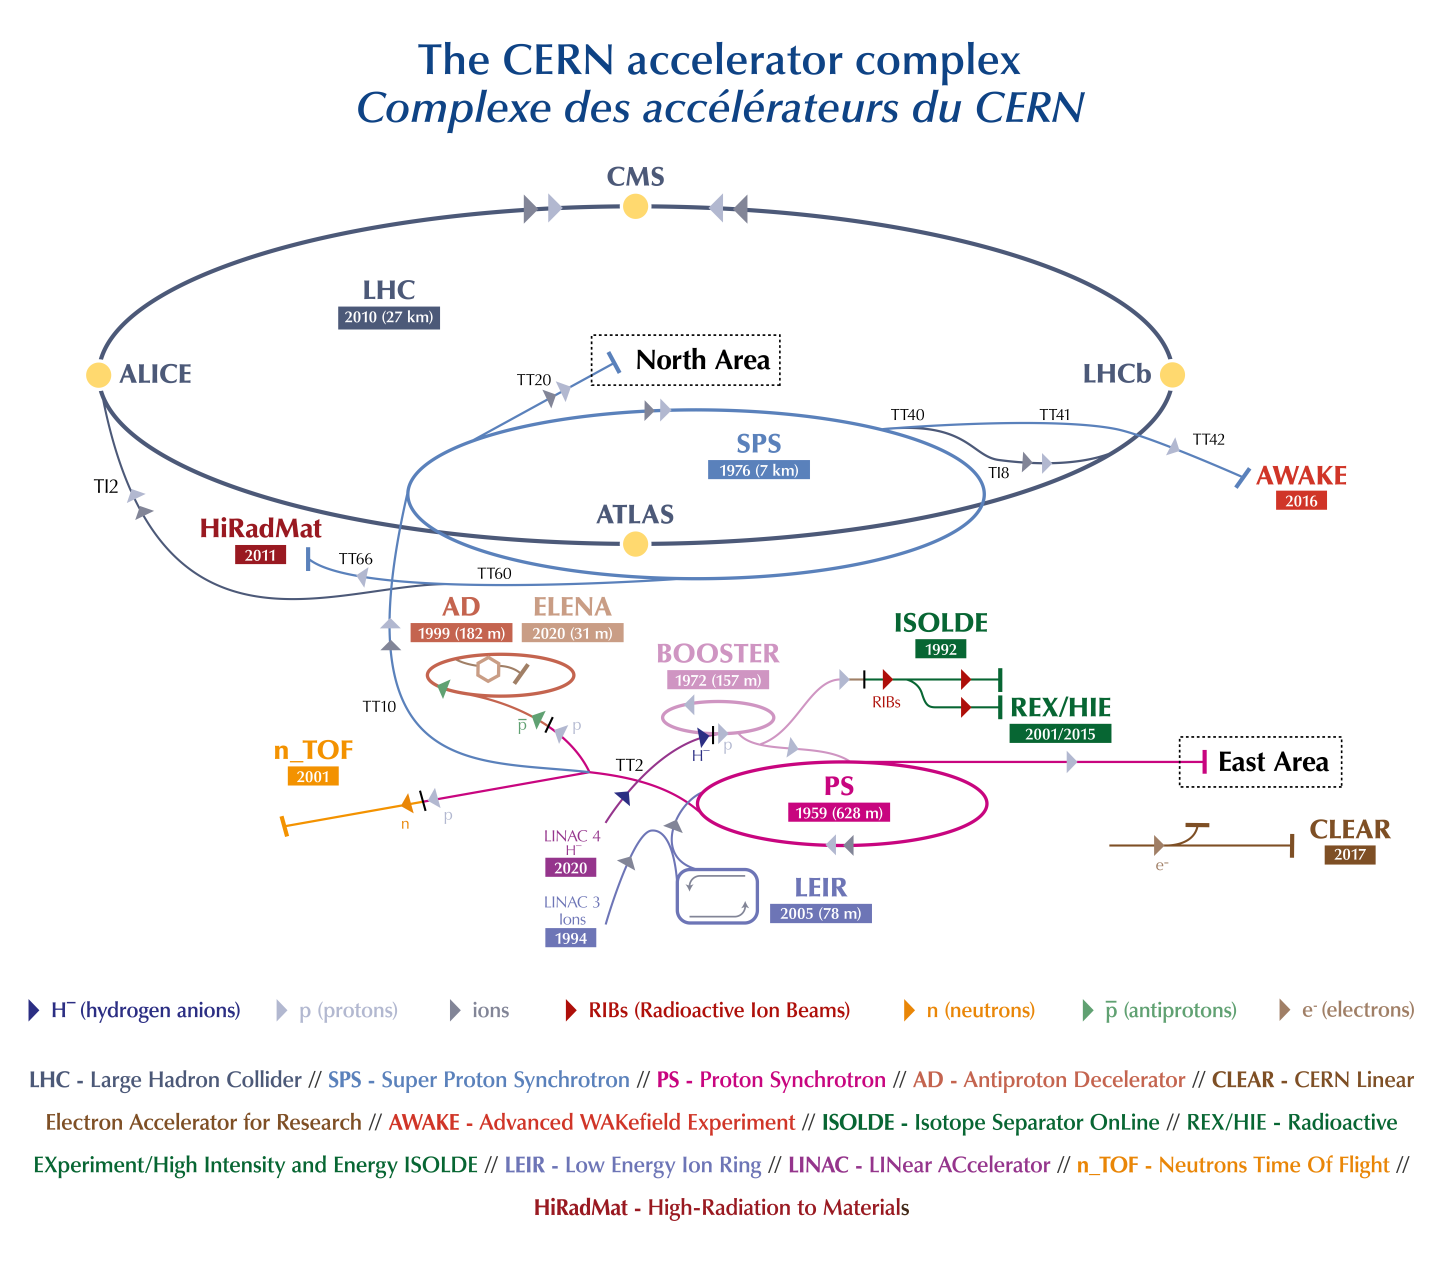
\includegraphics[width=\textwidth]{Figures/cern.png}
    \caption{A schematic diagram of the CERN  \cite{Bartosik:2847538}.}
    \label{fig:CERN_Schematic}
\end{figure}

The rate of events for a process produced in LHC collisions can be expressed as,

\begin{equation}
R_{\text{event}} = L_{\text{inst}} \sigma(\sqrt{s}), 
\end{equation}

where $\sigma$ represents the cross section of the process and is a function of the center-of-mass energy, and $L_{\text{inst}}$ denotes the LHC machine instantaneous luminosity, that depends only on the beam parameters and can be calculated by,

\begin{equation}
L_{\text{inst}} = \frac{n_{b}N_{b}^{2}f_{\text{rev}}\gamma_{r}}{4\pi \epsilon_{n}\beta^{*}}F.
\end{equation}

where $n_b$ is the number of bunches per beam, $N_b$ is the number of particles per bunch, $f_{\text{rev}}$ is the revolution frequency, $\gamma_r$ is the relativistic gamma factor, $\epsilon_n$ is the normalized transverse beam emittance, $\beta^*$ is the beta-function at the collision point, and $F$ is a reduction factor which accounts for the crossing angle of the beams at the collision point. 
One disadvantage of an increase the instantaneous luminosity is the increase of pileup (PU), defined as the number of additional inelastic proton-proton collisions per bunch crossing. \\

\begin{figure}[h]
    \centering
    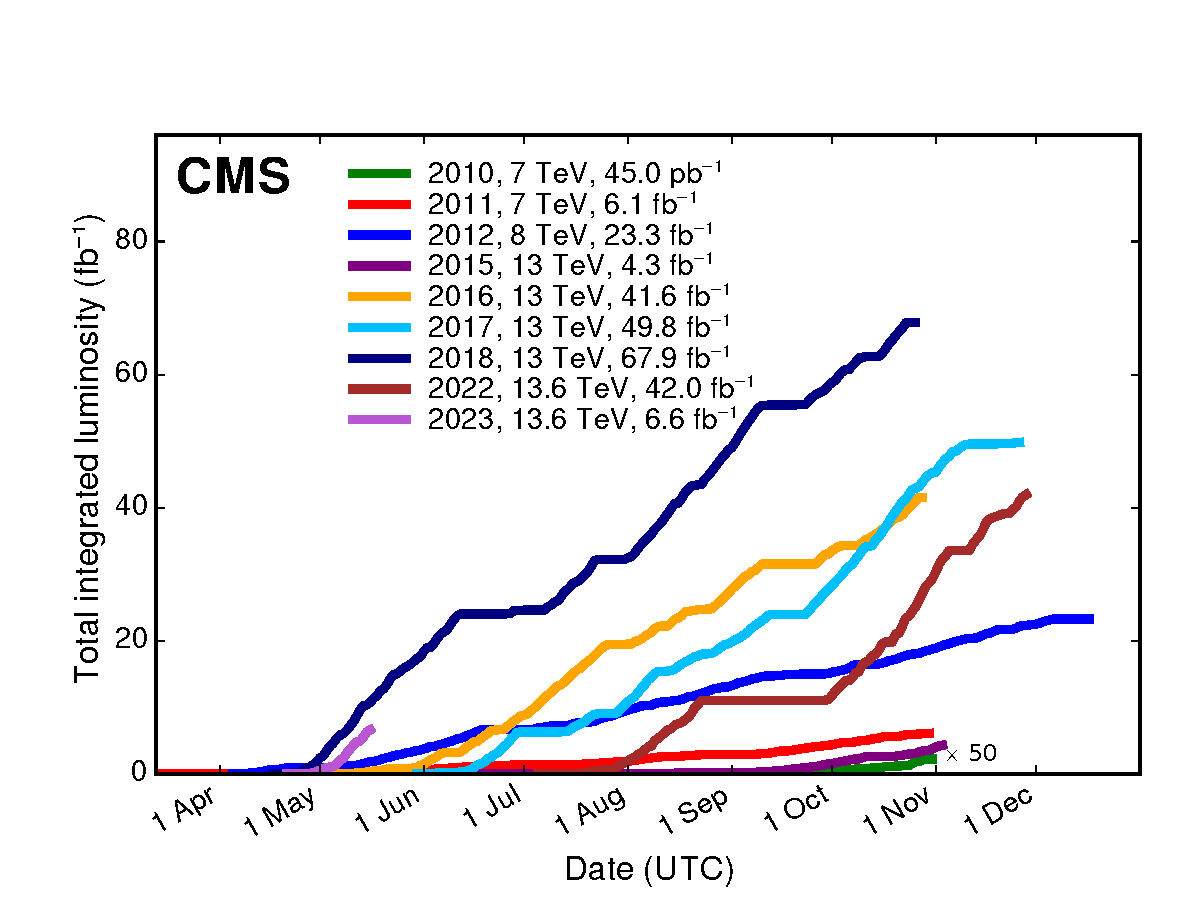
\includegraphics[width=0.9\textwidth]{Figures/int_lumi_cumulative_pp_2.pdf}
    \caption{The total integrated luminosity for proton-proton collisions collected by the CMS experiment between 2010 and May 2023~\cite{}.}
    \label{fig:int_lumi}
\end{figure}

The LHC began its first physics collisions in 2010, initially colliding beams at $\sqrt{s}$ = 7 TeV, which was increased to 8 TeV throughout 2012. 
Following this data-taking period, known as Run 1, the LHC underwent a two-year Long Shutdown 1 (LS1) to undergo upgrades in preparation for an increase in $\sqrt{s}$. 
In 2015, the LHC was restarted, initiating its Run 2 phase of data collection at $\sqrt{s}$ = 13 TeV, which lasted until the end of 2018. 
During Run 2, the LHC achieved and surpassed its original design luminosity by obtaining a record peak luminosity of $2.1\times10^{34}$ cm$^{−2}$s$^{−1}$ in 2018.
Subsequently, the LHC performed a second update period, the Long Shutdown 2 (LS2), lasting for approximately three years, where-after the data collection for Run 3 began at $\sqrt{s}$ = 13.6 TeV.
Fig~\ref{fig:int_lumi} illustrates the total integrated luminosity of proton-proton collisions delivered to the CMS detector at the time of writing.
The data used for the analyses described in this thesis correspond to the full Run 2 dataset collected during the 2016--2018 data-taking periods at 13 TeV. 
Only data recorded by CMS, where all sub-detectors were functioning correctly, are certified for use in physics analyses. 
This equates to 36.3 fb$^{−1}$, 41.5 fb$^{−1}$ and 59.7 fb$^{-1}$ of data collected in 2016, 2017 and 2018 respectively. \\

\section{The CMS Detector}

The Compact Muon Solenoid (CMS) detector was engineered to fulfil the rigorous demands of the LHC physics program. 
Its primary objective is to achieve sensitivity to the Higgs boson and novel phenomena at the TeV energy scale. 
Weighing 12,500 tonnes and measuring 21.6 m in length with a diameter of 14.6 m, the CMS detector uses an array of sub-detectors encircling the central beam axis. 
The layout of the CMS detector is shown in Fig.~\ref{fig:CMS_Schematic}.
A superconducting solenoid, operating at a magnetic field strength of 3.8 T, which encompasses the inner tracker, electromagnetic calorimeter, and hadronic calorimeter. 
Situated outside the solenoid within the iron return yoke are gaseous muon detectors, positioned to accurately measure muons. 
The CMS detector adopts a coordinate system centered at the collision point, with the y-axis oriented vertically, the x-axis directed radially inward toward the LHC center, and the z-axis aligned with the beam direction. Transverse energy ($E_T$) and transverse momentum ($\pT$) are defined in the x-y plane, and the azimuthal angle ($\phi$) and polar angle ($\theta$) are measured relative to the x-axis and z-axis, respectively. 
$r$ is used as the radial distance in the x-y plane.
Pseudorapidity ($\eta$), defined as $\eta = -\ln[\tan(\theta/2)]$, is used due to its gauge invariance, and distances in the $\phi$-$\eta$ plane are characterised by the metric $\Delta R = \sqrt{\Delta\phi^2 + \Delta\eta^2}$. 

\begin{figure}[h]
    \centering
    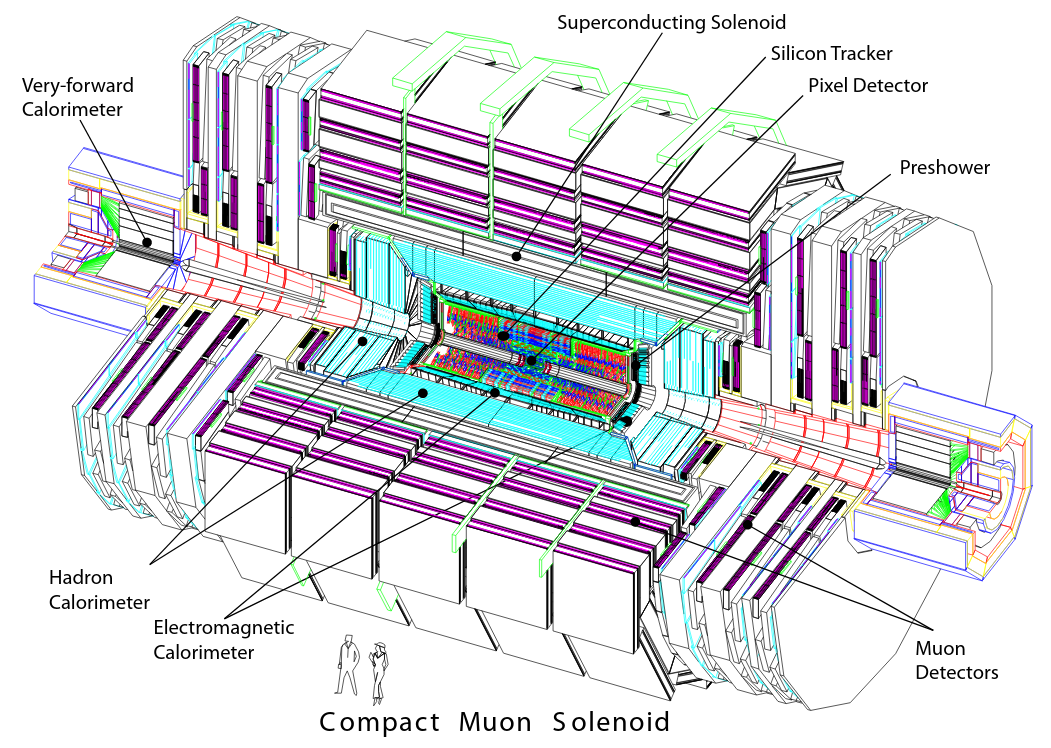
\includegraphics[width=0.9\textwidth]{Figures/CMS_Detector.png}
    \caption{A perspective view of the CMS detector \cite{CMS_Setup}.}
    \label{fig:CMS_Schematic}
\end{figure}

\subsection{Tracker}

Closest to the interaction point in the CMS experiment is the tracker~\cite{CMS_Setup,Malberti:2014pda,CMS:2012sda}, which is essential for precise measurements of charged particle trajectories and the determination of primary and secondary vertices. 
To meet the requirements of high granularity and fast response for the large number of particles generated in each bunch crossing, as well as being radiation-hard to deal with the particle flux, a silicon tracking detector is utilised. 
The tracker consists of a pixel detector and a silicon strip detector as shown in Fig.~\ref{fig:tracker}. \\

\begin{figure}[!hbtp]
    \centering
    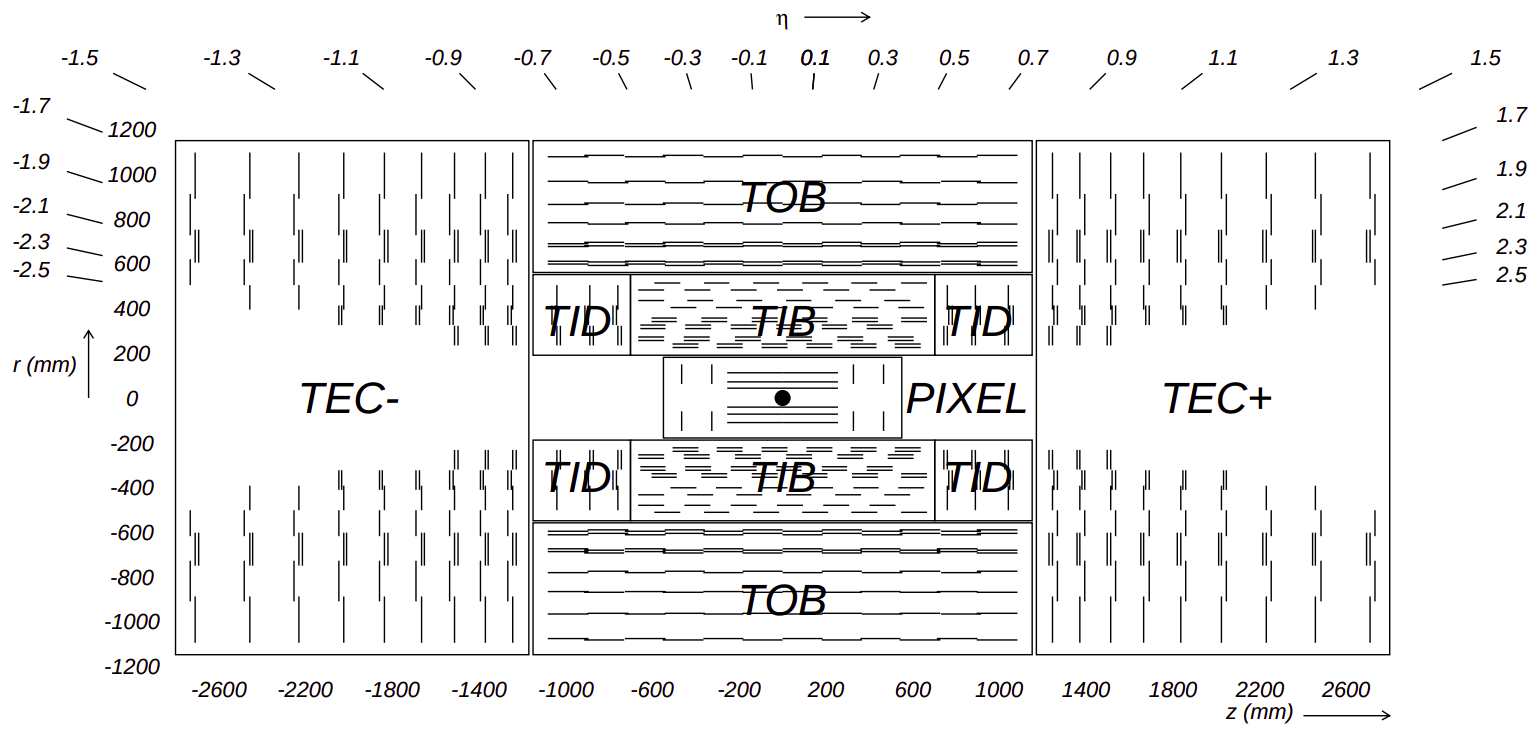
\includegraphics[width=\textwidth]{Figures/tracker.png}
    \caption{Schematic of the CMS tracker (pre-pixel upgrade) in the $r$-$z$ plane, showing the position of the pixel detector as well as the tracker inner barrel (TIB), tracker inner disks (TID), tracker outer barrel (TOB), and tracker endcaps (TEC) strip detectors. The lines represent detector modules and the double lines represent back-to-back modules~\cite{CMS_Setup}.}
    \label{fig:tracker}
\end{figure}

The pixel detector covers the pseudorapidity range $|\eta| < 2.5$ and is composed of three cylindrical pixel modules and two disk pixel modules. 
It contains 66 million silicon pixels, each with dimensions of $100 \times 150$ $\mu$m${^2}$. 
This configuration provides a spatial resolution of $15-20$ $\mu$m in both the $r$-$\phi$ plane and the $z$ direction, enabling 3-dimensional vertex reconstruction.
The original tracker was built to handle as instantaneous luminosity of $10^{34}$ cm$^{2}$s$^{-1}$ and an average PU of 25.
To handle higher luminosities and increased event PU, the pixel detector was upgraded in 2016/2017 to handle approximately double the instantaneous luminosity and PU~\cite{CMS:2012sda}. 
The upgraded detector consists of four barrel module layers and three endcap disks, resulting in 124 million pixels. \\

Surrounding the pixel detector is the silicon strip detector, which is divided into four subsystems: the tracker inner barrel (TIB), tracker inner disks (TID), tracker outer barrel (TOB), and tracker endcaps (TEC). 
The TIB and TID provide four layers of silicon strip detectors in the barrel region and three disks at each end, extending up to a radius of 55 cm. 
The TOB consists of six barrel layers extending up to an outer radius of 116 cm, while the TEC comprises nine disks covering a range of $|z|$ from 124 cm to 282 cm. 
The silicon strips have various thickness and widths, providing multiple measurements of the $r$-$\phi$ position with resolutions ranging from 23-35 $\mu$m in the TIB to 35-53 $\mu$m in the TOB. \\

In addition to the main components, the tracker includes back-to-back mounted micro-strip detector modules to provide additional measurements of the $z$ coordinate in specific regions. 
The overall tracker layout ensures the presence of at least three hits in the pixel detector (at least four hits for the upgraded detector) and at least nine hits in the silicon-strip tracker, with a minimum of four 2-dimensional measurements among them.

\subsection{Electromagnetic calorimeter}

The CMS electromagnetic calorimeter (ECAL) is a hermetic homogeneous calorimeter designed to detect high-energy electrons and photons~\cite{CMS_Setup,CMS:2013lxn}. 
In total, 75,848 lead tungstate (PbWO$_4$) crystals are sorted in a barrel and endcap configuration. 
PbWO$_4$ was chosen as the crystal material due to its radiation-hardness, high density, short radiation length, and small Molière radius (the average radius containing on average 90\% of
a shower’s total energy deposit), enabling the construction of a compact and finely granular ECAL. 
Scintillation light produced by showering electrons and photons in the crystals is converted into an electrical signal by photodetectors such as avalanche photodiodes in the barrel and vacuum phototriodes in the endcaps. 
The scintillation decay time of the crystals matches the 25 ns LHC bunch crossing time, ensuring that a significant portion of the light is emitted between bunch crossings. \\

The ECAL is placed outside of the tracker but within the magnet bore and covers the pseudorapidity range $|\eta| < 3.0$. 
It comprises of an ECAL barrel (EB) covering $|\eta| < 1.479$ and an ECAL endcap (EE) covering $1.479 < |\eta| < 3.0$. 
A diagram of this is shown in Fig.~\ref{fig:ecal}.
The barrel region consists of 61,200 crystals with 360-fold granularity in $\phi$ and ($2 \times 85$)-fold granularity in $\eta$. 
The crystals are tapered with a front face area of $0.0174 \times 0.0174$ in $\eta$-$\phi$ ($22 \times 22$ mm$^2$) and a length of 230 mm. 
The endcaps house 7,324 crystals arranged in a rectangular $x$-$y$ grid, each with a front face area of $28.62 \times 28.62$ mm$^2$ and a length of 220 mm. \\

The ECAL system also includes Preshower detectors placed in front of each endcap to identify photons from neutral pion decays and improve electron identification and position resolution. 
These detectors consist of lead radiators to initiate showering and silicon-strip sensors to measure the deposited energy. 
The ECAL energy resolution is parametrized as a function of the incident particle energy (E), with terms for the stochastic (S), noise (N), and constant (C) contributions.

\begin{equation}
\Big(\frac{\sigma}{E}\Big)^2 = \Big(\frac{S}{\sqrt{E}}\Big)^2 + \Big( \frac{N}{E} \Big) + C^2
\end{equation}

The stochastic term captures fluctuations in lateral shower containment and photon yield, the noise term accounts for electronics noise and pileup, and the constant term arises from non-uniformity of the longitudinal response and calibration errors. 
Measurements using electron beams have determined the values of S = 0.028 GeV$^{1/2}$, N = 0.12 GeV, and C = 0.003 for the ECAL energy resolution. \\

\begin{figure}[!hbtp]
    \centering
    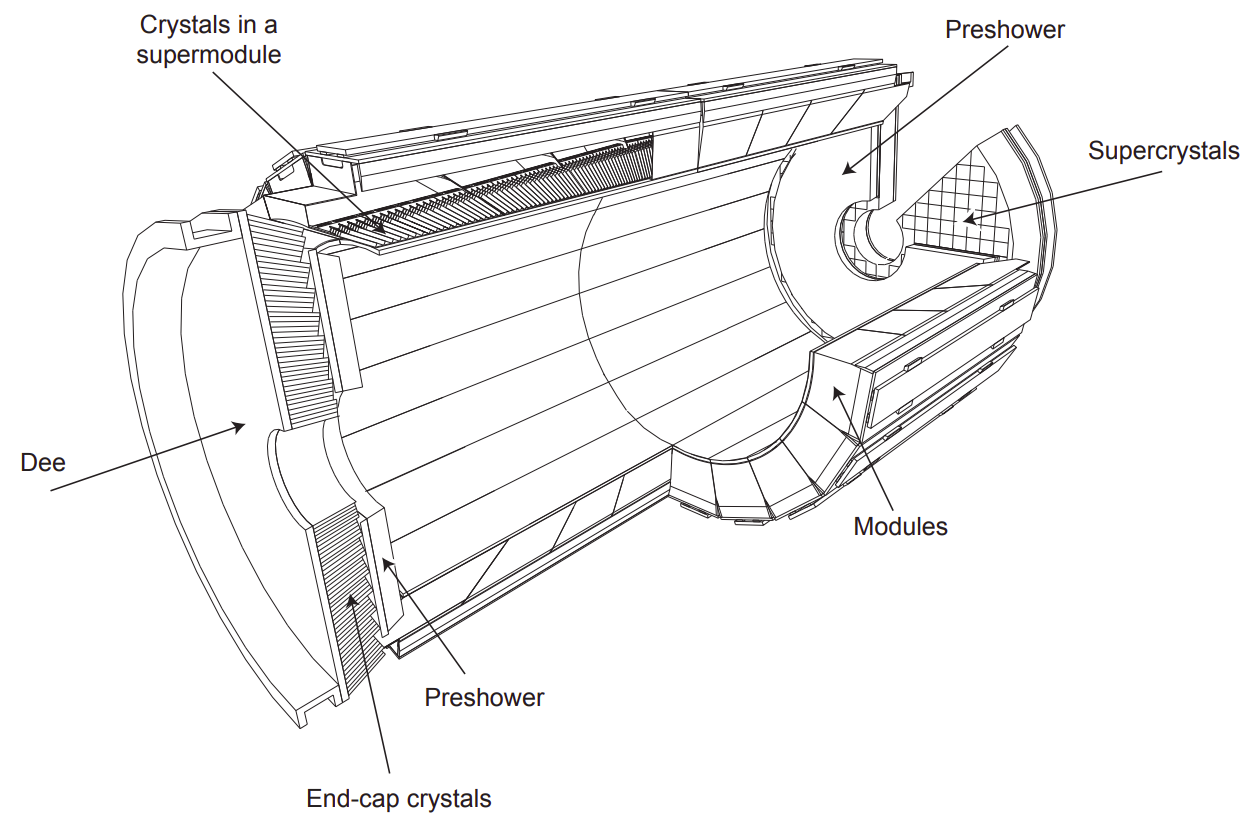
\includegraphics[width=\textwidth]{Figures/ECAL.png}
    \caption{A schematic of the CMS ECAL detector~\cite{CMS_Setup}.}
    \label{fig:ecal}
\end{figure}

\subsection{Hadron calorimeter}

\begin{figure}[!hbtp]
    \centering
    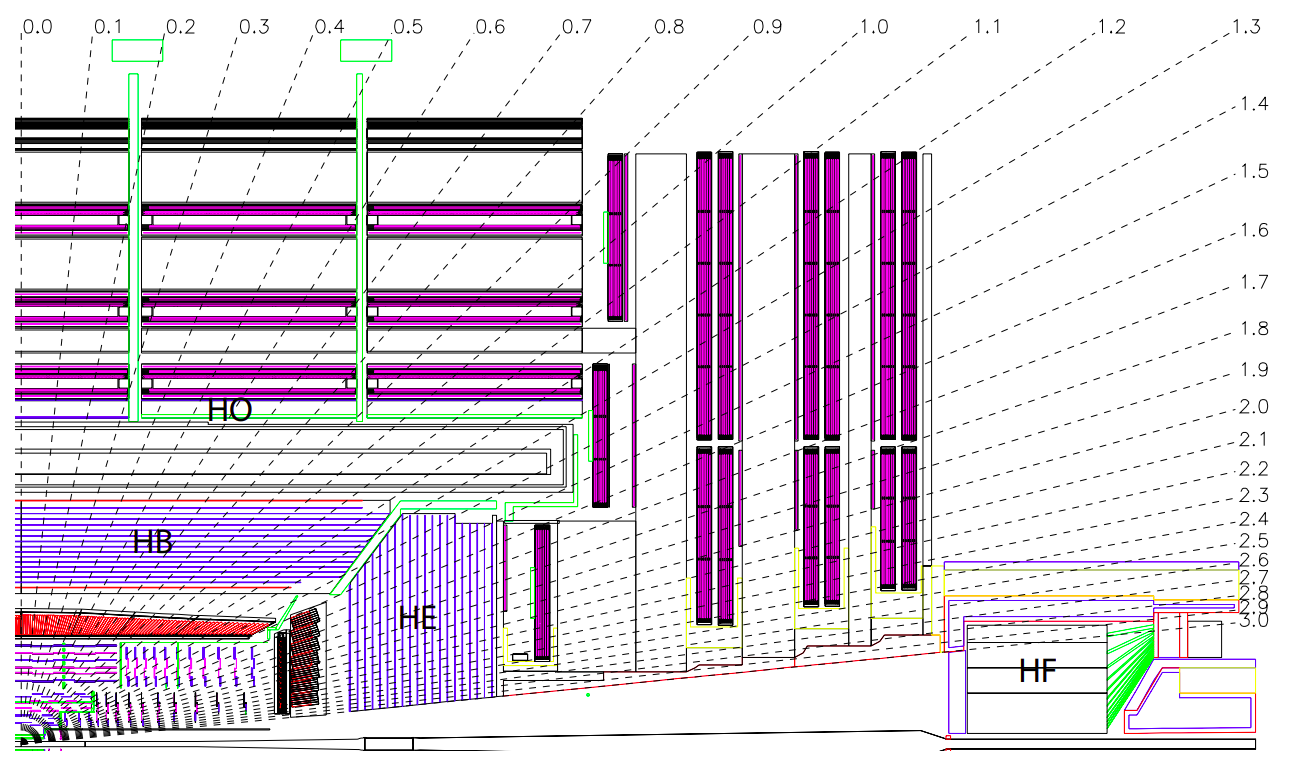
\includegraphics[width=\textwidth]{Figures/HCAL.png}
    \caption{.}
    \label{fig:}
\end{figure}

\subsection{Muon system}
\subsection{Triggering}

